\documentclass{article}
\usepackage{tikz,pgfplots}
\usepackage{tikz-qtree}
\usepackage{units}
\pgfplotsset{compat=1.8}
%\pgfplotsset{colormap={mix}{
%	color(0cm)=(blue);
%	color(1cm)=(green);
%	color(2cm)=(yellow)
%	color(3cm)=(red)}}

\usetikzlibrary{patterns,shadows,trees}

\definecolor{diplom1}{rgb}{0.0 0.4 1.0}
\definecolor{diplom2}{rgb}{0.0 0.0 0.6}
\definecolor{diplom3}{RGB}{153,0,0} %unirot
\definecolor{diplom4}{RGB}{232,215,23}
\definecolor{diplom5}{RGB}{51,37,60}

\definecolor{unirot}{RGB}{153,0,0}
\definecolor{unirot_hell}{RGB}{255,228,225}
\definecolor{lightblue}{RGB}{242.2,249.88,255}

\pgfplotsset{colormap={diplom1s}{
       color(0cm)=(white);
       color(1cm)=(diplom1);
       color(10cm)=(diplom1)}}
\pgfplotsset{colormap={diplom2s}{
       color(0cm)=(white);
       color(1cm)=(diplom1);
       color(2cm)=(diplom2)}}
\pgfplotsset{colormap={blues}{
       color(0cm)=(diplom2);
       color(1cm)=(diplom1);
       color(2cm)=(white);
       color(3cm)=(diplom1);
       color(4cm)=(diplom2)}}


\begin{document}

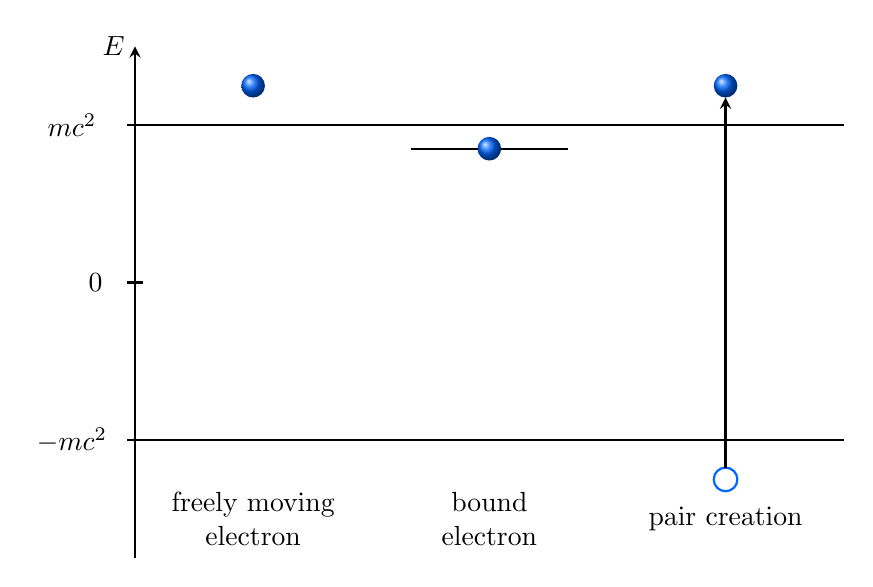
\begin{tikzpicture}[
          scale=1.0,>=stealth
        ]
%     \tiny
 % \draw[very thin,color=gray] (-0.1,-4.1) grid (10.9,4.9);
 \draw [->, thick] (0,-3.5) -- (0,3) node [left]{$E$};
 \draw [thick] (-0.1,-2) -- (9,-2);
 \node at (-0.8,-2) {$-mc^2$};
 \draw [thick] (-0.1,2) -- (9,2);
 \node at (-0.8,2) {$mc^2$};
 \draw [thick] (-0.1,0) -- (0.1,0);
 \node at (-0.5,0) {0};

 \shade [ball color=diplom1] (1.5,2.5) circle (0.15);
 \node [align=center] at (1.5,-3) {freely moving\\electron};

 \draw [thick] (3.5,1.7) -- (5.5,1.7);
 \shade [ball color=diplom1] (4.5,1.7) circle (0.15);
 \node [align=center] at (4.5,-3) {bound\\electron};

 \shade [ball color=diplom1] (7.5,2.5) circle (0.15);
 \draw [thick,diplom1] (7.5,-2.5) circle (0.15);
 \draw [thick,->] (7.5,-2.35) -- (7.5,2.35);
 \node [align=center] at (7.5,-3) {pair creation};

\end{tikzpicture}

\end{document}
